\documentclass[11pt]{article}

\usepackage{epsfig}
\usepackage{amsfonts}
\usepackage{amssymb}
\usepackage{amstext}
\usepackage{amsmath}
\usepackage{xspace}
\usepackage{theorem}
\usepackage{hyperref}
\usepackage{fullpage}
%\usepackage[]{algorithm2e}
\usepackage{xfrac}
\usepackage{mathtools}
\usepackage{algorithm}
\usepackage{algpseudocode}

\usepackage{listings}

\DeclarePairedDelimiter\ceil{\lceil}{\rceil}
\DeclarePairedDelimiter\floor{\lfloor}{\rfloor}

\usepackage{enumitem}                     

\usepackage{tikz}
\usepackage{tikz-qtree}
\usetikzlibrary{arrows,shapes,snakes,automata,backgrounds,petri,decorations.markings}

\tikzstyle{code} = [black!90, draw=black!30, fill=black!5, very thick,
    rectangle, dashed, inner xsep=10pt, inner ysep=7pt]

\newenvironment{codebox}{
    \hspace{.05\textwidth}
        \begin{tikzpicture}
            \node[code] \bgroup
                \begin{minipage}{.65\textwidth}
                    \begin{alltt}}
                    {\end{alltt}
                \end{minipage}
            \egroup;
        \end{tikzpicture}
}

\newif\ifrubric
\rubrictrue
 
 
 
 \usepackage{titlesec}

\titleformat*{\section}{\bfseries}
\titleformat*{\subsection}{\bfseries}
\titleformat*{\subsubsection}{\bfseries}
\titleformat*{\paragraph}{\bfseries}
\titleformat*{\subparagraph}{\bfseries}


\newenvironment{proof}{{\bf Proof:  }}{\hfill\rule{2mm}{2mm}}
\newenvironment{proofof}[1]{{\bf Proof of #1:  }}{\hfill\rule{2mm}{2mm}}
\newenvironment{proofofnobox}[1]{{\bf#1:  }}{}
\newenvironment{example}{{\bf Example:  }}{\hfill\rule{2mm}{2mm}}

\newtheorem{fact}{Fact}
\newtheorem{lemma}[fact]{Lemma}
\newtheorem{theorem}[fact]{Theorem}
\newtheorem{definition}[fact]{Definition}
\newtheorem{corollary}[fact]{Corollary}
\newtheorem{proposition}[fact]{Proposition}
\newtheorem{claim}[fact]{Claim}
\newtheorem{exercise}[fact]{Exercise}

% math notation
\newcommand{\R}{\ensuremath{\mathbb R}}
\newcommand{\Z}{\ensuremath{\mathbb Z}}
\newcommand{\N}{\ensuremath{\mathbb N}}
\newcommand{\F}{\ensuremath{\mathcal F}}
\newcommand{\SymGrp}{\ensuremath{\mathfrak S}}

\newcommand{\size}[1]{\ensuremath{\left|#1\right|}}
%\newcommand{\ceil}[1]{\ensuremath{\left\lceil#1\right\rceil}}
%\newcommand{\floor}[1]{\ensuremath{\left\lfloor#1\right\rfloor}}
\newcommand{\poly}{\operatorname{poly}}
\newcommand{\polylog}{\operatorname{polylog}}

% anupam's abbreviations
\newcommand{\e}{\epsilon}
\newcommand{\half}{\ensuremath{\frac{1}{2}}}
\newcommand{\junk}[1]{}
\newcommand{\sse}{\subseteq}
\newcommand{\union}{\cup}
\newcommand{\meet}{\wedge}

\newcommand{\prob}[1]{\ensuremath{\text{{\bf Pr}$\left[#1\right]$}}}
\newcommand{\expct}[1]{\ensuremath{\text{{\bf E}$\left[#1\right]$}}}
\newcommand{\Event}{{\mathcal E}}
\newcommand{\E}{\ensuremath{\text{E}}}

\newcommand{\mnote}[1]{\normalmarginpar \marginpar{\tiny #1}}
\newcommand{\opt}[0]{{\text{OPT}}}

\setenumerate[0]{label=(\alph*)}


%%%%%%%%%%%%%%%%%%%%%%%%%%%%%%%%%%%%%%%%%%%%%%%%%%%%%%%%%%%%%%%%%%%%%%%%%%%
% Document begins here %%%%%%%%%%%%%%%%%%%%%%%%%%%%%%%%%%%%%%%%%%%%%%%%%%%%
%%%%%%%%%%%%%%%%%%%%%%%%%%%%%%%%%%%%%%%%%%%%%%%%%%%%%%%%%%%%%%%%%%%%%%%%%%%



\begin{document}

\noindent {\large {\bf 601.433/633 Introduction to Algorithms} \hfill {{\bf Fall 2026}}}\\ 
{{\bf Homework \#9}} \hfill {{\bf Due:} December 3, 2026, 11:59pm} \\
\rule[0.1in]{\textwidth}{0.4pt}

Remember: you may work in groups, but must write up your solution entirely on your own. Solutions must by typeset (\LaTeX\ preferred but not required). 
Collaboration is limited to discussing the problems -- you may not look at, compare, reuse, etc.~any text from anyone else in the class. 
You may use the internet to look up formulas, definitions, etc., but may not simply look up the answers online.  

Please include proofs with all of your answers, unless stated otherwise.


\noindent \rule[0.1in]{\textwidth}{0.4pt}

\section{Circulations (33 points)}

Let's look at some variations of max-flow. In class, we talked about algorithms to compute the maximum flow from a source $s$ to a sink $t$ 
in a directed graph $G= (V, E)$ when we are given edge capacities $c : E \rightarrow \mathbb{R^+}$. A valid flow was a function 
$f : E \rightarrow \mathbb{R}_{\geq 0}$ so that $f(e) \leq c(e)$ for all $e \in E$, and for all nodes $v \in V \setminus\{s,t\}$ 
we required the flow in to equal the flow out, i.e.~$\sum_{u} f(u,v) = \sum_{u} f(v,u)$.

\begin{enumerate}
\item (16 points) What if we no longer have a single $s$ and a single $t$? Instead, think of every node $v$ as having a demand $d_v$. 
If $d_v$ is positive then $v$ wants flow; it is a sink. If $d_v$ is negative then $v$ wants to get rid of flow; it is a source. 
And if $d_v = 0$ then $v$ wants to simply transit flow; it is neither a source nor a sink. A valid \emph{circulation} is an assignment 
$f : E \rightarrow \mathbb{R}_{\geq 0}$ such that $f(e) \leq c(e)$ for all $e \in E$ (i.e., capacities are not violated), 
and $\sum_{u} f(u,v) - \sum_{u} f(v,u) = d_v$ for all $v \in V$ (i.e., at every node the flow-in minus the flow-out is equal to the demand).

Given a directed graph with capacities and demands, give a polynomial-time algorithm to determine whether a valid circulation exists. 
Prove correctness and polynomial running time. Hint: reduce to max-flow.

\bigbreak

\textbf{Algorithm Description:}

TODO

\bigbreak

\textbf{Correctness Proof:}

TODO

\bigbreak

\textbf{Runtime Proof:}

TODO

\bigbreak

\item (17 points) Let's make things even more complicated. Capacities are an upper bound on flow -- we are not allowed to send more flow through an edge 
than its capacity allows.  What if we also want to have lower bounds? That is, in addition to capacities $c$, we are also given lower bounds 
$\ell : E \rightarrow \mathbb{R}_{\geq 0}$ and we require $\ell(e) \leq f(e) \leq c(e)$ for all $e \in E$?

Let's redefine a valid circulation with these lower bounds. We are now given a directed graph $G = (V,E)$, capacities $c : E \rightarrow \mathbb{R}^+$, 
lower bounds $\ell : E \rightarrow \mathbb{E}_{\geq 0}$, and for each vertex $v$ we are given a demand $d_v$. A valid circulation is now a function 
$f : E \rightarrow \mathbb{R}_{\geq 0}$ such that $\ell(e) \leq f(e) \leq c(e)$ for all $e \in E$, and $\sum_{u} f(u,v) - \sum_{u} f(v,u) = d_v$.

Give a polynomial-time algorithm to determine whether a valid circulation exists. Prove correctness and polynomial running time. 

Hint: Try to transform the problem into finding a circulation without lower bounds, i.e., the setting of part (a). You might want to start by 
initially setting $f(e)= \ell(e)$ for all $e$. This will not be a valid circulation, but what does the "remaining" problem look like?

\bigbreak

\textbf{Algorithm Description:}

TODO

\bigbreak

\textbf{Correctness Proof:}

TODO

\bigbreak

\textbf{Runtime Proof:}

TODO

\end{enumerate}


\section{Realizable Degree Sequences (33 points)}

Recall that the \emph{in-degree} of a vertex $v$ in a directed graph is the number of edges that go into $v$, i.e.~the number of edges of the form $(u,v)$. 
Similarly, the \emph{out-degree} is the number of edges leaving $v$, i.e.~the number of edges of the form $(v,u)$. Let $d_{v,in}$ denote the 
in-degree of $v$, and let $d_{v,out}$ denote the out-degree. In this problem we will not allow any loops (edges of the form $(u,u)$) 
or multiedges (i.e.~any edge $(u,v)$ can only be in the graph at most once, although both $(u,v)$ and $(v,u)$ could be in the graph).

\begin{enumerate}
\item  (16 points)
Suppose you are given the following set of degree constraints for a four-node directed graph:
\begin{align*}
&d_{1,in} = 0, d_{1,out} = 2 \\
&d_{2,in} = 1, d_{2,out} = 2 \\
&d_{3,in} = 1, d_{3,out} = 1 \\
&d_{4,in} = 3, d_{4,out} = 0
\end{align*}

Is there a directed graph, with no multi-edges or self-loops, that satisfies these constraints?  If so, what is it?  If not, why not?

\bigbreak

Yes, there is a graph that satisfied these constraints.

\medbreak

\textbf{Adjacency list:}

$1 \rightarrow [2, 4]$

$2 \rightarrow [3, 4]$

$3 \rightarrow [4]$

$4 \rightarrow []$

\medbreak

\textbf{Representation:}

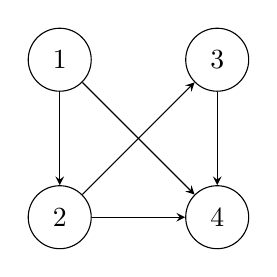
\begin{tikzpicture}[->, >=stealth, node distance=2cm, every node/.style={circle, draw, minimum size=8mm}]
    \node (1) at (0, 0) {1};
    \node (2) at (0, -2) {2};
    \node (3) at (2, 0) {3};
    \node (4) at (2, -2) {4};

    \draw (1) -- (2);
    \draw (1) -- (4);
    \draw (2) -- (3);
    \draw (2) -- (4);
    \draw (3) -- (4);
\end{tikzpicture}

\bigbreak

\item (17 points) This type of specification, where we are given the in- and out-degrees of every vertex, is called a \emph{degree sequence}. 
The question above was whether a particular degree sequence is \emph{realizable} -- that is, whether there exists a graph having those degrees.

Give a polynomial-time algorithm that, given a degree sequence, will determine if it is realizable, and if it is will produce a directed graph 
with those degrees. The graph should not have any self loops or multi-edges (i.e., for each directed pair $(i,j)$ with $i \neq j$ there can be 
at most one edge from $i$ to $j$, although it is fine if there is also an edge from $j$ to $i$). Prove that your algorithm is correct, 
and runs in polynomial time.

Hint: think flow, and think about creating a useful auxiliary graph.

\bigbreak

\textbf{Algorithm Description:}

First, we perform a simple check where for the degrees given, we define:

$$D = \sum_{j=1}^{n} d_j^{out}$$

Then, we ensure that the following holds true:

$$D = \sum_{j=1}^{n} d_j^{in}$$

If there is a mismatch in the total out degree and total in degree, then sequence cannot work, so we return \texttt{False}.

Now, we create an auxiliary structure in the form of a bipartite graph where each vertex is duplicated. Thus, for each vertex $j$ in the original graph, 
our bipartite graph has left-side vertex $o_j$ and right-side vertex $i_j$, representing outgoing edges of $j$ and incoming edges of $j$, respectively. 
Next, we connect all possible edges within the constraints, so for all $u, v$ such that $u \neq v$, we add $(o_u, i_v)$ to the graph with capacity $1$. 
We perform an intermediary check here to allow for early termination, where we check if the number of edges in the bipartite graph is less than $D$. 
In this case, there are not enough possible edges to saturate the needed out-degree requirement, so we can return \texttt{False}.

This graph can then be turned into a flow network. We add source $s$, with an outgoing edge to all outgoing edges $o_j$, where the capacity of 
each $(s, o_j)$ is equal to the out-degree of $j$, and destination $t$, where all incoming edges $I$ have an outgoing edge to $t$. 
We use Edmonds-Karp to then find the maximum flow over the auxiliary structure from $s$ to $t$. Let $M$ be the maximum flow found by Edmonds-Karp.

Now that we have this structure, we can determine whether the given degree sequence is realizable over these nodes. 
Recall variable $D$, representing the total out-degree of the original graph. From here, we have 2 cases:

\begin{enumerate}[label=(\arabic*), noitemsep]
    \item $D < M$ -- There are not enough possible outgoing edges over those nodes to reach the needed overall out-degree. 
    Thus, the sequence is not realizable. Algorithm returns \texttt{False}
    \item $D = M$ -- There are enough outgoing edges to reach the overall out-degree. The sequence is realizable.
    \item Note that $D > M$ is impossible by the max-flow/min-cut theorem, as the minimum cut across the graph is equal to $D$, 
    so the max flow found by Edmonds Karp can be no greater.
\end{enumerate}

Now that we know the sequence is realizable, we turn to the creation of th\texttt{False}.e directed graph with the given degree sequence. 
We initialize an empty graph $G$ where vertices $V$ are the $n$ original given vertices nd $E = \emptyset$.
We then iterate over every edge between the left and right side of the auxiliary maximum flow network. 
For any edge in the auxiliary network $(o_u, i_v)$, we add edge $(u, v)$ to $G$. 
This produces a graph with the given degree sequence.

\bigbreak

\textbf{Correctness Proof:}

To prove correctness, we must prove that the algorithm returns a graph with the given degree sequence if and only if such a graph exists. 
We will do so by proving both directions of this statement.

\medbreak

First, we prove the statement: if a graph with the given degree sequence exists, the algorithm returns it. 
We assume such a graph $G$ exists. We will first show that the maximum flow $M$ found in the auxiliary graph has a value equal to $D$. 
When adding each edge $(s, o_j)$ for each vertex $j$, we set the capacity of that edge to the out-degree of vertex $j$. 
When adding each edge $(i_j, t)$ for each vertex $j$, we set the capacity of that edge to the in-degree of vertex $j$. 
Since we know $D \leq \text{num. edges in the bipartite graph}$, the cut between left and right side has capacity at least $D$, 
and the cuts between $s$ and the rest of the graph and $t$ and the rest of the graph have capacity exactly $D$. 
Thus, the minimum cut of the auxiliary structure is $D$, so the maximum flow of the structure is $D$. 

Now, we show that the maximum flow produced is equal to the given degree sequence when the graph is assembled to prove the correct graph is returned. 
Since the maximum flow has a value of $D$, all edges leaving the source and entering the sink must be saturated. 
This means that each vertex $o_j$ sends exactly $d_j^{out}$ units of flow, and each vertex $i_k$ receives exactly $d_k^{in}$ units of flow. 
Furthermore, since all edges between the left and right sides of the bipartite graph have a capacity of $1$, and the maximum flow is integral, 
each edge carries either $0$ or $1$ units of flow. To construct the original graph, we iterate through each edge $(o_i, i_j)$ in the bipartite graph. 
If the edge carries 1 unit of flow, we add the corresponding directed edge $(i, j)$ to our original graph. Otherwise, we do nothing.

Since each vertex $o_j$ sends exactly $d_j^{out}$ units of flow, the corresponding vertex $j$ in our original graph has exactly $d_j^{out}$ outgoing edges. 
Similarly, since each vertex $i_k$ receives exactly $d_k^{in}$ units of flow, the corresponding vertex $k$ in our original graph has 
exactly $d_k^{in}$ incoming edges. Additionally, since we do not create edges between $o_j$ and $i_j$, there are no self-loops, 
and since each edge between the two sides has a capacity of $1$, there are no multi-edges.

Therefore, the graph constructed by our algorithm has exactly the given degree sequence and satisfies the required restrictions.

\medbreak

Next, we prove the statement: if the algorithm returns a graph with the given degree sequence, then such a graph exists. 
We prove this by contrapositive, so we will prove: if no graph with the given degree sequence exists, the algorithm does not return a graph. 
We assume that no graph with the given degree sequence exists. We assume FTSOC that the algorithm returns a graph with the given degree sequence. 
As per the argument above, we know that if the algorithm returns a graph, then $M = D$. Since the total capacity leaving $s$ and entering $t$ is both $D$, 
every edge leaving the source and every edge entering the sink must be saturated. Because the capacities between the left and right sides 
are $1$ and the flow is integral, every such edge carries either $0$ or $1$ unit of flow. In the graph constructed by the algorithm, 
every edge $(o_u, i_v)$, we add $(u, v)$ to $G$. By the proof above, we know each vertex $u$ has $d_u^{out}$ outgoing edges. 
Thus, exactly $d_u^{out}$ edges enter the incoming vertices. Since $(i_u, t)$ is saturated, we know $d_u^{in}$ edges enter $i_u$, 
so $u$ has $d_u^{in}$ incoming edges. Because $(o_u, i_u)$ was not included for all $u$, there are no self-loops. 
Because every edge between the sides has capacity $1$, there are no multi-edges. Therefore, $G$ has precisely the specified degree sequence. 
This contradicts the assumption that no such graph exists. Thus, if no graph with the given degree sequence exists, the algorithm cannot return a graph.
In proving the contrapositive, we prove the original statement.

\medbreak

Therefore, in proving the $2$ parts of the original statement, we prove that the algorithm is correct.

\bigbreak

\textbf{Runtime Proof:}

We will follow the steps of the algorithm to find the total running time of this algorithm. 

First, the initial degree check iterates over every vertex, keeping track of out-degree and in-degree, giving a runtime of $O(n)$ for this step. 
Next, we create the bipartite graph. We must initialize adjacency lists for each of the $2n$ vertices, taking $O(2n) = O(n)$ time.  
We then add edges for each of the viable vertices, keeping track of how many edges we add. Thus, for each of the $n$ outgoing vertices, 
we iterate over the $n$ incoming vertices to check if we can add an edge, giving runtime $n * O(n) = O(n^2)$. 
From here, we add the source and sink, along with their respective edges to each of the outgoing and incoming vertices. 
This is another iteration over each of the vertices twice, giving time $O(2n) = O(n)$. 

Now, we run Edmonds-Karp. As per \textbf{Theorem 20.3.4}, the runtime is $O(m^{2}n)$. However, we can simplify this further. 
We added any edge $(o_u, i_v)$ to the auxiliary graph provided $u \neq v$. Therefore, each of the $n$ outgoing vertices has $n-1$ edges. 
Furthermore, there are $n$ edges $(s, o_j)$ and $n$ edges $(i_j, t)$. Summing this, we know the auxiliary graph has a total number of edges: 
$m = n * (n-1) + n + n = n^2 - n + 2n = n^2 + n = O(n^2)$. Therefore, the runtime of Edmonds-Karp is $O(m^{2}n) = O(((n)^{2})^{2}n) = O(n^5)$ . 

Finally, for the final step where create the directed graph, we must initialize $n$ adjacency lists first. 
We then iterate through the max-flow graph, and add an edge $(u, v)$ for each $(o_u, i_v)$ in the flow graph. 
As the maximum viable number of out-edges is $O(n * (n-1)) = O(n^2)$, this step takes at most $O(n^2)$ time. 

Summing, we have a total runtime of:

$$O(n) + O(n) + O(n^2) + O(n) + O(n^5) + O(n^2)$$

Clearly, the $O(n^5)$ term dominates the others, giving a simplified runtime of:

$$O(n^5)$$

\end{enumerate}


\section{Linear Programming (34 points)}

Let's consider linear programming formulations of the maximum-weight matching problem. We now have an (undirected) graph $G = (V, E)$ 
and weights $w : E \rightarrow \mathbb{R}^+$ (note that we \emph{are not} assuming that $G$ is bipartite). Our goal is to find the matching $M$ which 
maximizes $\sum_{e \in M} w(e)$, under the constraint that for all $e, e' \in M$, $e \cap e' = \emptyset$ (that is, no two edges in $M$ share an endpoint).  

Consider the following linear program which has a variable $x_e$ for every edge $e$.

\begin{align*}
\max &\sum_{e \in E} w(e) x_e \\
\text{subject to} & \sum_{v : \{u,v\} \in E} x_{\{u,v\}} \leq 1  & \forall u \in V \\
& x_e \geq 0 & \forall e \in E
\end{align*}


\begin{enumerate}
\item (17 points) Prove that the optimal value of this LP is \emph{at least} the weight of the maximum-weight matching.

\bigbreak

TODO

\bigbreak

\item (17 points) Unlike the examples in class, this is not an exact formulation of the maximum-weight matching problem. 
Find a graph $G = (V,E)$ and weights $w : E \rightarrow \mathbb{R}^+$ such that the optimal LP value is strictly larger than the weight of 
the maximum-weight matching (and prove this).

\bigbreak

TODO

\end{enumerate}

\end{document}
